\section{Methodology}
\begin{frame}{Methodology Overview}
  \begin{itemize}
    \item \textbf{System Architecture Design}
      \begin{itemize}
        \item Flutter-based mobile application
        \item Spring back-end for authentication and data management
        \item Llama 3.2 integration with RAG capabilities
      \end{itemize}
    \item \textbf{Doc2Conv Development}
      \begin{itemize}
        \item Multi-agent system for conversation generation
        \item Integration with multiple LLM providers
        \item Chain-of-thought reasoning implementation
      \end{itemize}
    \item \textbf{Model Fine-tuning}
      \begin{itemize}
        \item Dataset preparation from generated conversations
        \item qLoRA fine-tuning of Llama 3.2
        \item Evaluation metrics for performance assessment
      \end{itemize}
  \end{itemize}
\end{frame}

\begin{frame}{Doc2Conv: Multi-Agent Cluster for Synthetic Dialogue Corpus Generation}
  \begin{columns}[T]
    \begin{column}{0.45\textwidth}
      \begin{itemize}
        \item Transforms static document content into dynamic, interactive conversations
        \item Leverages multiple LLM providers through a unified interface
        \item Employs specialized agents for different aspects of conversation generation
        \item Facilitates domain-specific knowledge transfer
      \end{itemize}
    \end{column}
    
    \begin{column}{0.55\textwidth}
      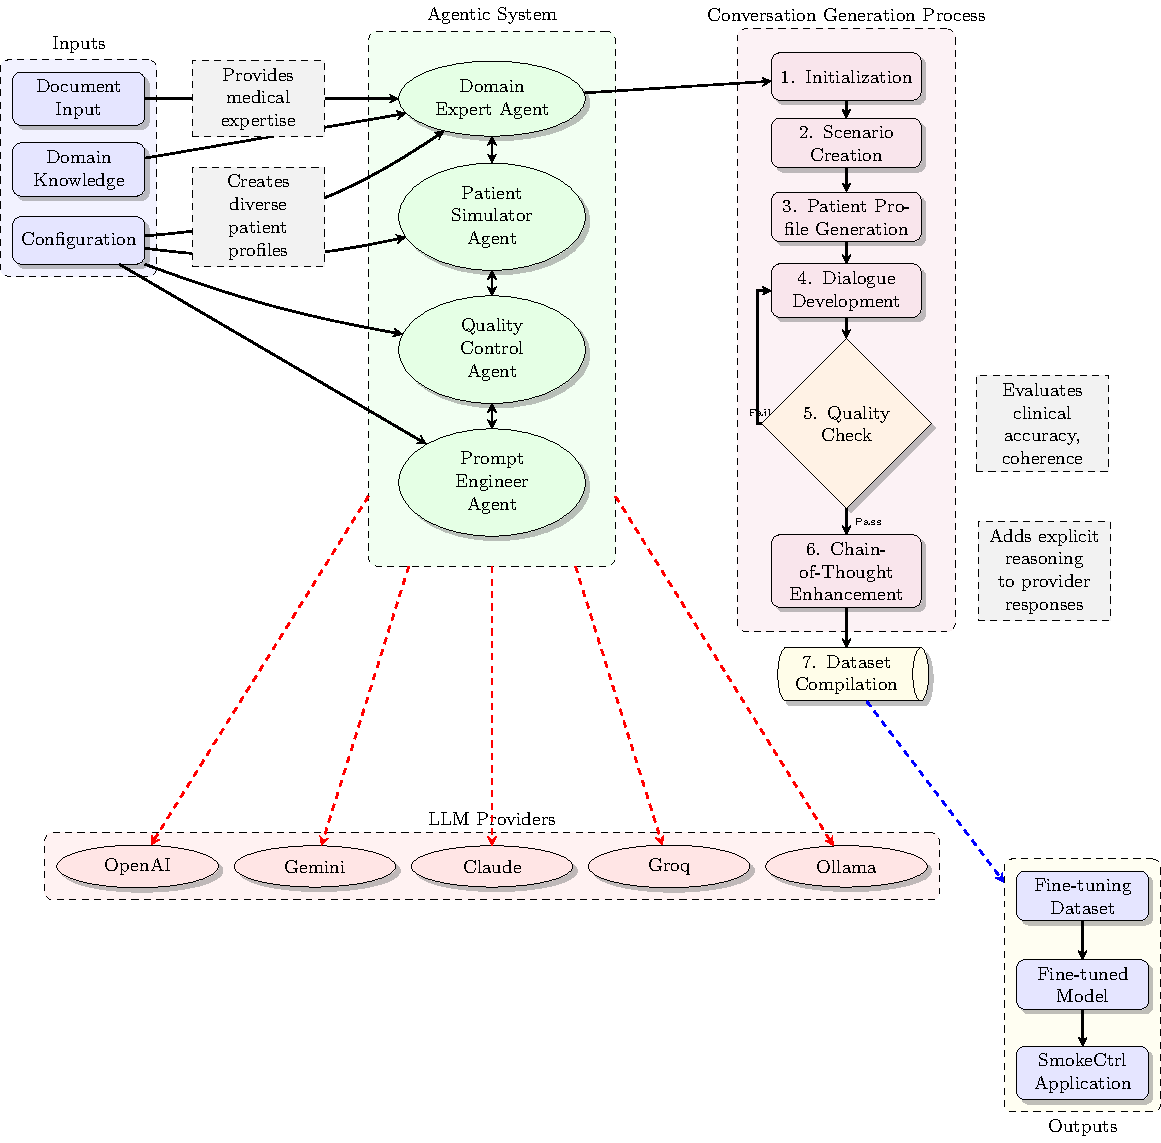
\includegraphics[width=\textwidth, height=0.62\paperheight]{presentation/images/Pictures/doc2conv_architecture.pdf}
    \end{column}
  \end{columns}
\end{frame}

\begin{frame}{Synthetic Dialogue Corpus Generation: Methodological Framework}
  \begin{columns}
    % Left column with bullet points
    \begin{column}{0.5\textwidth}
      \begin{itemize}
        \item Multi-phase generative pipeline with iterative quality validation protocols
        
        \item Explicit reasoning pathway elicitation through metacognitive prompting techniques
        
        \item Stochastic diversity mechanisms ensuring representational heterogeneity
        
        \item Domain-constrained semantic validation ensuring clinical fidelity
      \end{itemize}
    \end{column}

    % Right column with image
    \begin{column}{0.5\textwidth}
      \begin{center}
        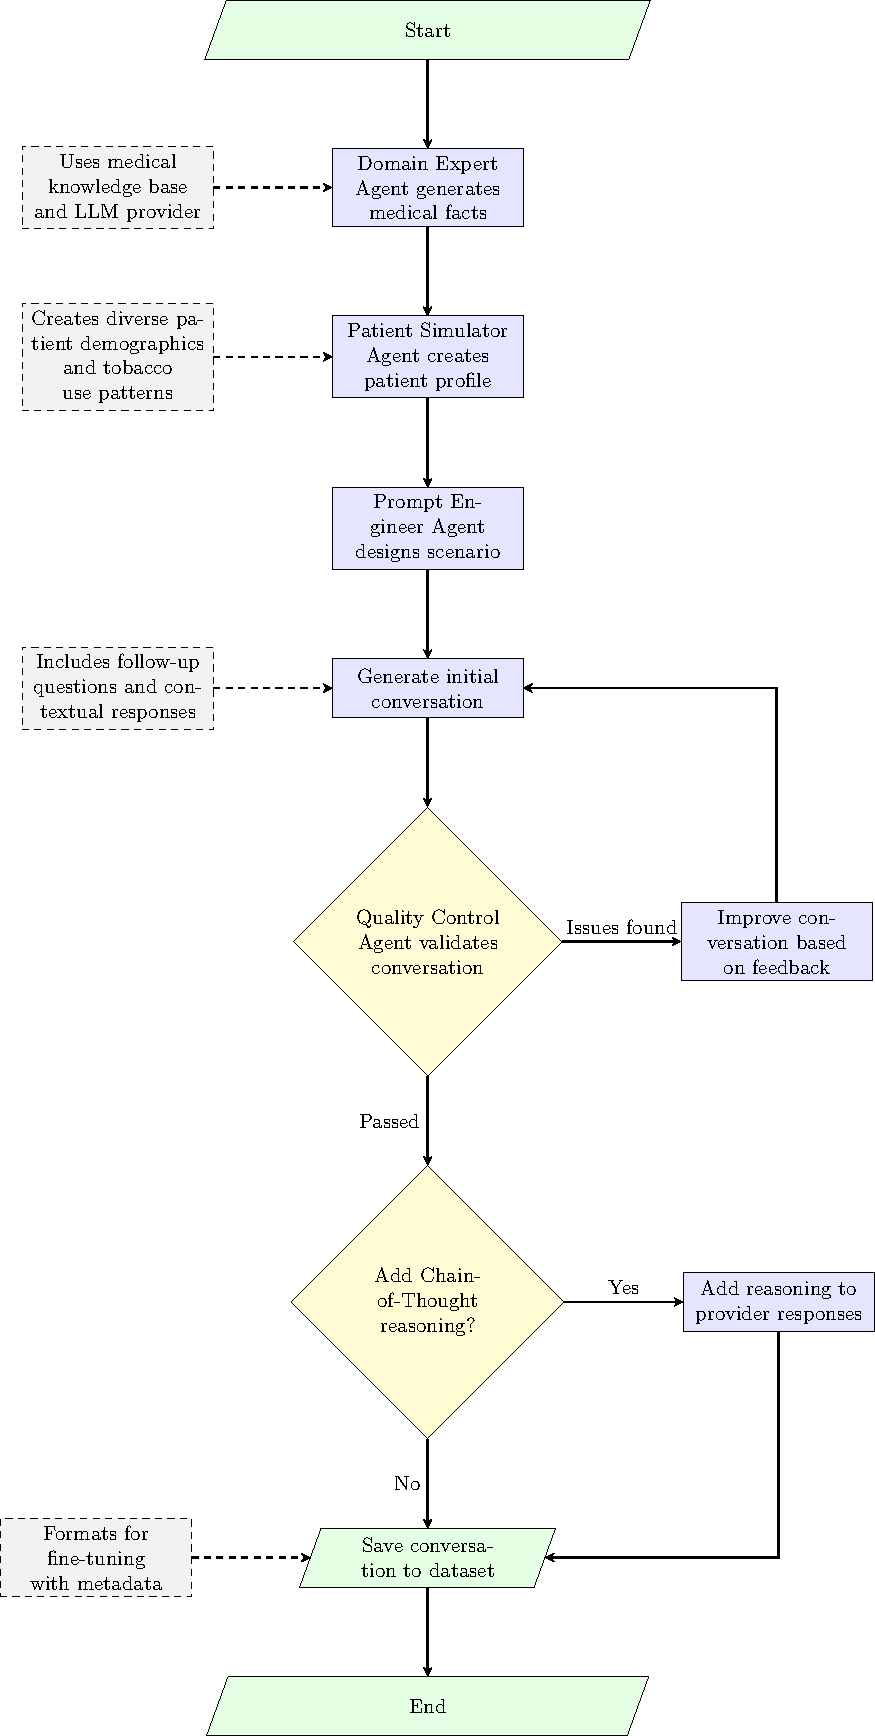
\includegraphics[width=0.75\textwidth, height=0.70\paperheight]{presentation/images/Pictures/conversation_generation_flow.pdf}
      \end{center}
    \end{column}
  \end{columns}
\end{frame}